% Hvor hurtig var min implementation i forhold til basismodellen?
% Hvor præcis var min implementation i forhold til hvad man kan forvente? Hvor meget variede svaret i forhold til den forventede værdi?
% Variede mit svar på forskellige maskiner?
\subsection{Results}
\begin{figure}
    \centering
    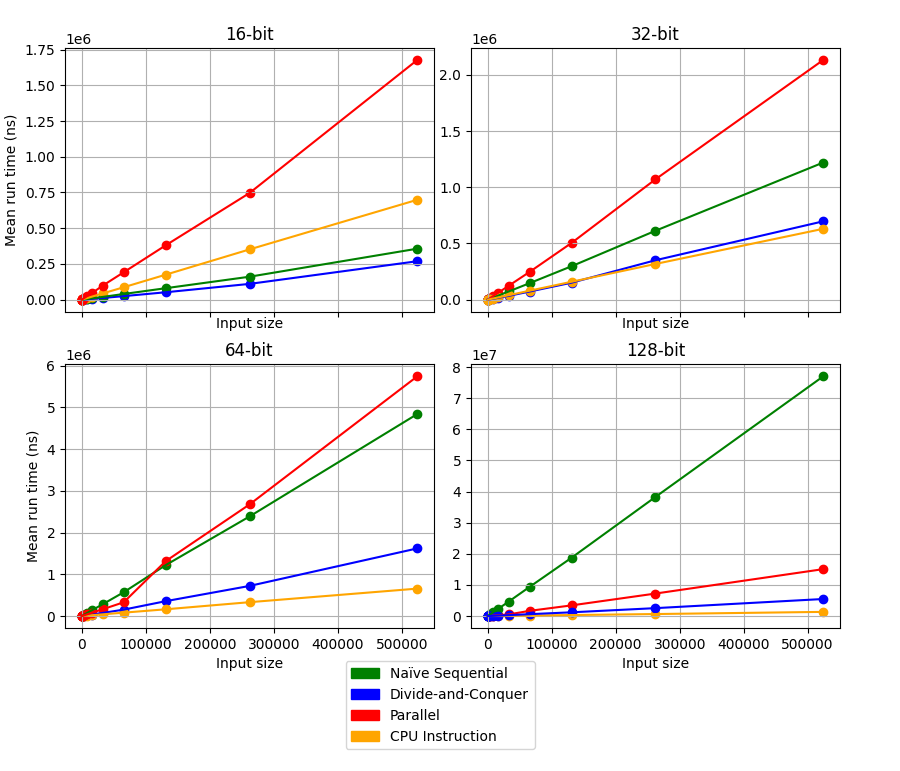
\includegraphics[width=\textwidth]{combined.png}
    \caption{Execution time of each algorithm on different word sizes}
    \label{fig:runningtime}
\end{figure}
The benchmarks were run on different input sizes that were all powers of two - in this case $\{2^4, 2^5, \dots 2^{19}\}$ and with word sizes $\{16, 32, 64, 128\}$. The results can be seen in figure \ref{fig:runningtime}. 
It can be seen that the parallel algorithm is significantly slower for small word sizes, and only becomes more efficient than the naïve sequential algorithm when $w=128$. This must mean that the hidden factors hidden in the big-O notation of the parallel algorithm's time complexity outweigh the $w$ factor of the naïve algorithm. This makes sense, since the parallel algorithm is much more complex and only starts benefiting from parallelism after the first three iterations. Interestingly enough, when $w=64$, the parallel algorithm only seems to be slower when the input size is larger than $2^{16}$. This can be due to the input data being able to fit inside 128 KiB L1 data cache on my machine (see appendix A for machine specifications).\\
When run on 128-bit size words, the naïve sequential algorithm performs much worse than both the parallel and the divide-and-conquer algorithm. This shows that when we increase the word size, algorithms that have a linear dependency on $w$ suffer much more than algorithms that have a logarithmic dependency, which is as expected.\\
It is also seen that the divide and conquer algorithm significantly outperforms both the parallel and the naïve algorithm at all word sizes. This is might be due to the fact that it is much simpler than the parallel algorithm and is asymptotically more optimal than the naïve sequential algorithm.
The final thing to note is that the \texttt{popcnt} CPU instruction is the ultimately fastest option out of the algorithms. This shows that these algorithms might only be useful on hardware that does not support this instruction or on very large word sizes. Even then, the divide-and-conquer algorithm seems to be sufficiently efficient for many uses or even superior to the parallel algorithm despite its sub-optimal theoretical running time.\\

